\documentclass[11pt]{article}
\usepackage{amsmath}
\usepackage{fourier}
\usepackage{fullpage}
\usepackage{graphicx}
\usepackage[colorlinks = true,
            linkcolor = blue,
            urlcolor  = blue,
            citecolor = blue,
            anchorcolor = blue]{hyperref}
\usepackage{epigraph}
\usepackage{wrapfig}
\usepackage{fancyhdr}

\pagestyle{fancy}
\fancypagestyle{plain}{
    \fancyhf{}
    \lfoot{© 2021 Ben Grant. Some rights reserved (\href{https://creativecommons.org/licenses/by-sa/4.0/}{CC BY-SA 4.0}).}
    \rfoot{\thepage}
    \renewcommand{\headrulewidth}{0pt}
}
\fancyhf{}
\lfoot{© 2021 Ben Grant. Some rights reserved (\href{https://creativecommons.org/licenses/by-sa/4.0/}{CC BY-SA 4.0}).}
\rfoot{\thepage}
\renewcommand{\headrulewidth}{0pt}

% syntax highlighting style by Eugene Chou

\usepackage[most]{tcolorbox}

\definecolor{cblack}{HTML}{161616}
\definecolor{cgray}{HTML}{676767}
\definecolor{cred}{HTML}{FD4285}
\definecolor{cgreen}{HTML}{A6E22D}
\definecolor{cyellow}{HTML}{E5DA72}
\definecolor{corange}{HTML}{FD9720}
\definecolor{cblue}{HTML}{0094D8}
\definecolor{cmagenta}{HTML}{9A37FF}
\definecolor{ccyan}{HTML}{50B6D8}
\definecolor{cwhite}{HTML}{C7C7C7}

\lstloadlanguages{C,C++,make,python,fortran,bash}

\newtcolorbox{prelab}[1]{
  colback=red!5!white, colframe=red!75!black, title=#1
}

\newcommand\Warning{%
 \makebox[1.4em][c]{%
 \makebox[0pt][c]{\raisebox{.1em}{\small!}}%
 \makebox[0pt][c]{\color{red}\Large$\bigtriangleup$}}}%

\lstdefinestyle{c99}{
  language=C++,
  upquote=true,
  backgroundcolor=\color{cblack},
  emphstyle=\color{ccyan},
  emph={
    int,
    void,
    char,
    long,
    float,
    double,
    signed, unsigned
    int8_t, int16_t, int32_t, uint64_t,
    uint8_t, uint16_t, uint32_t, uuint64_t,
  },
  keywordstyle=\color{cred},
  keywordstyle=[2]\color{cgreen},
  morekeywords=[2]{main,printf,getopt,random,srandom,scanf,fprintf,puts},
  stringstyle=\color{cyellow},
  directivestyle=\color{cmagenta},
  commentstyle=\color{cgray},
  identifierstyle=\color{cwhite},
  numberstyle=\ttfamily\color{corange},
  basicstyle=\footnotesize\ttfamily\color{cwhite},
  breakatwhitespace=false,
  breaklines=true,
  captionpos=b,
  keepspaces=true,
  showspaces=false,
  showstringspaces=false,
  showtabs=false,
  numbers=left,
  numbersep=7pt,
  xleftmargin=10pt,
  tabsize=4
}

\lstdefinestyle{python}{
  language=python,
  upquote=true,
  backgroundcolor=\color{cblack},
  keywordstyle=\color{cred},
  keywordstyle=[2]\color{cgreen},
  morekeywords=[2]{main,print,sqrt},
  stringstyle=\color{cyellow},
  commentstyle=\color{cgray},
  identifierstyle=\color{cwhite},
  numberstyle=\ttfamily\color{corange},
  basicstyle=\footnotesize\ttfamily\color{cwhite},
  breakatwhitespace=false,
  breaklines=true,
  captionpos=b,
  keepspaces=true,
  showspaces=false,
  showstringspaces=false,
  showtabs=false,
  numbers=left,
  numbersep=7pt,
  xleftmargin=10pt,
  tabsize=4
}

\lstdefinestyle{bash}{
  language=bash,
  upquote=true,
  backgroundcolor=\color{cblack},
  keywordstyle=\color{cwhite},
  keywordstyle=[2]\color{cwhite},
  morekeywords=[2]{main,print,sqrt},
  stringstyle=\color{cyellow},
  commentstyle=\color{cgray},
  identifierstyle=\color{cwhite},
  basicstyle=\footnotesize\ttfamily\color{cwhite},
  numbers=none,
  breakatwhitespace=false,
  breaklines=true,
  captionpos=b,
  keepspaces=true,
  showspaces=false,
  showstringspaces=false,
  showtabs=false,
  xleftmargin=-5pt,
  tabsize=4
}

\newtcblisting{clisting}[2][]{
  title=#2, #1,
  fonttitle=\footnotesize\bfseries,
  colframe=black!75,
  colback=cblack,
  listing only,
  listing options={style=c99},
  top=-5pt,
  bottom=-5pt,
  enlarge top by=5pt
}

\newtcblisting{pylisting}[2][]{
  title=#2, #1,
  fonttitle=\footnotesize\bfseries,
  colframe=black!75,
  colback=cblack,
  listing only,
  listing options={style=python},
  top=-5pt,
  bottom=-5pt,
  enlarge top by=5pt
}

\newtcblisting{shlisting}[2][]{
  title=#2, #1,
  fonttitle=\footnotesize\bfseries,
  colframe=black!75,
  colback=cblack,
  listing only,
  listing options={style=bash},
  top=-5pt,
  bottom=-5pt,
  enlarge top by=5pt
}

\title{
    Assignment 8 \\
    Touch Grass
}
\author{
    Ben Grant \\
    CSE 13S -- Fall 2021
}
\date{
    First \texttt{DESIGN.pdf} draft due: December 69$^\text{th}$ at 11:59\,pm PST \\
    Assignment due: December 420$^\text{th}$ at 11:59\,pm PST \\
    Up-to-date headers, binary, and PDF at \url{https://github.com/190n/asgn8}
}

\begin{document}\maketitle
\section{Introduction}

\setlength{\epigraphwidth}{0.76\textwidth}
\epigraph{\emph{If you want to relax, watch the clouds pass by if you're laying on the grass, or sit in front of the creek; just doing nothing and having those still moments is what really rejuvenates the body.}}{---Miranda Kerr}

\begin{wrapfigure}{r}{0.4\textwidth}
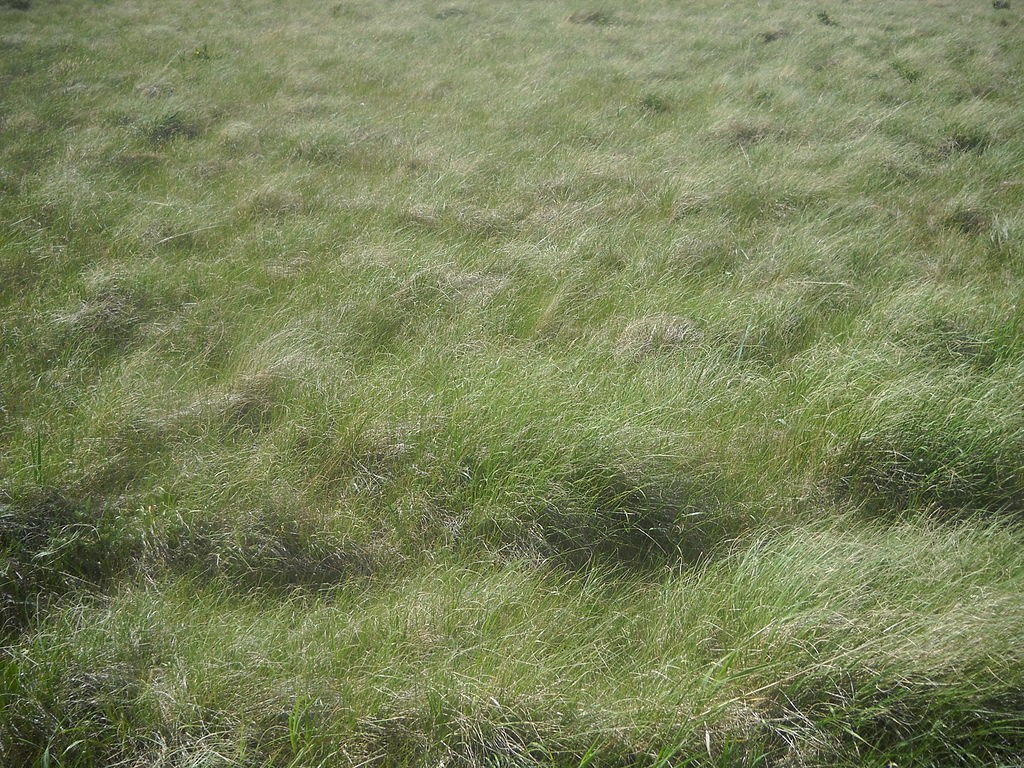
\includegraphics[width=0.4\textwidth]{field}
A grassy field. Image by Dustin V.S. via \href{https://commons.wikimedia.org/wiki/File:Grasses_in_the_Valles_Caldera_2014-06-26.JPG}{Wikimedia Commons}. \href{https://creativecommons.org/licenses/by-sa/3.0/deed.en}{CC BY-SA 3.0}.
\end{wrapfigure}

\noindent
Grass is one of the most prevalent types of plants on Earth. While most would picture a grassy lawn or field (see image) when they think of grass, common staples like wheat, rice, and corn are also grasses.

While grass has been known and touched throughout human history, the phrase ``touch grass'' has recently gained new meaning. It's used as an insult, suggesting that its target is hung up on something meaningless (especially on the Internet) and should go outside.

Those of you that have actually touched grass may know that blades of grass can be flattened with very little force, and may remain that way for some time. In this assignment, we will create data structures to represent a field of grass, and investigate several methods for flattening the entire field as quickly as possible.

\section{Is this all a joke?}

\setlength{\epigraphwidth}{0.46\textwidth}
\epigraph{\emph{Of course it is happening inside your head, Harry, but why on earth should that mean that it is not real?}}{---Albus Dumbledore}
\setlength{\epigraphwidth}{0.76\textwidth}

\noindent
Of course this is a joke. Now let us continue with the assignment --- grass does not touch itself!

\section{Bit Vectors}

\epigraph{\emph{Rest is not idleness, and to lie sometimes on the grass under trees on a summer's day, listening to the murmur of the water, or watching the clouds float across the sky, is by no means a waste of time.}}{---John Lubbock, \emph{The Use of Life}}

\begin{wrapfigure}[14]{l}{0.4\textwidth}
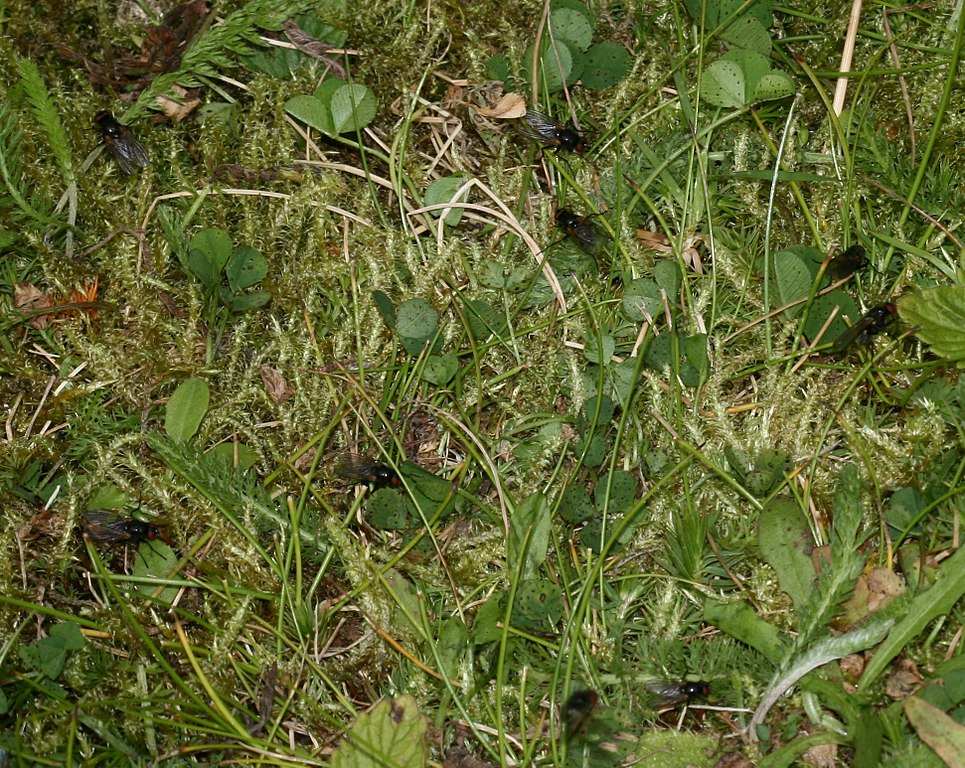
\includegraphics[width=0.4\textwidth]{flat}
Flattened blades of grass. Image by \href{https://www.flickr.com/people/35142635@N05}{S. Rae} via \href{https://commons.wikimedia.org/wiki/File:Hydrotaea_sp\%5E_on_flattened_grass_patch_-_Flickr_-_S._Rae.jpg}{Wikimedia Commons}. \href{https://creativecommons.org/licenses/by/2.0}{CC BY 2.0}.
\end{wrapfigure}

\noindent
A single blade of grass has two states: standing or flattened. This lends itself well to representation via a bit vector, as each bit also has two states.

``But Ben,'' you say (performance-sensitive programmer that you are), ``surely this is inefficient! I have a 64-bit CPU (to say nothing of AVX and friends), so why must I touch only one blade at a time?''

In this assignment, we make an important change to the bit vector: we store the vector as an array of 64-bit integers instead of an array of bytes. This will allow us to set 64 bits at once and hopefully speed up our code. We also add a field to track how many times the bit vector has been written to, in order to quantify this speedup. Here is the \texttt{struct} definition:

\begin{clisting}{}
struct BitVector {
    uint32_t length;
    uint64_t *vector;
    uint32_t writes;
};
\end{clisting}

This \texttt{struct} definition \emph{must} go in \texttt{bv.c}.

\setlength{\parindent}{0pt}
\setlength{\parskip}{6pt}

\underline{\texttt{BitVector *bv\_create(uint32\_t size)}}

The constructor for a bit vector. \texttt{size} is the number of bits in the vector. \texttt{writes} should be initialized to zero. The vector itself should also be filled with zeros.
\medskip

\underline{\texttt{void bv\_delete(BitVector **bv)}}

The destructor for a bit vector. All memory should be freed and the pointer set to \texttt{NULL}.
\medskip

\underline{\texttt{uint32\_t bv\_length(BitVector *bv)}}

Get the length of a bit vector.
\medskip

\underline{\texttt{bool bv\_set\_bit(BitVector *bv, uint32\_t i)}}

If \texttt{i} is a valid index into the bit vector, set that bit to one and return \texttt{true}. Otherwise, return \texttt{false}. For this and the other functions that access the bit vector, you must be careful with your bitwise arithmetic since the vector stores 64-bit values. Without casting, integer literals may default to 32 bits, and this can cause operations to be performed incorrectly.
\medskip

\underline{\texttt{bool bv\_clr\_bit(BitVector *bv, uint32\_t i)}}

If \texttt{i} is a valid index into the bit vector, set that bit to zero and return \texttt{true}. Otherwise, return \texttt{false}.
\medskip

\underline{\texttt{bool bv\_get\_bit(BitVector *bv, uint32\_t i, bool *bit)}}

If \texttt{i} is a valid index into the bit vector, store the indicated bit in \texttt{*bit} and return \texttt{true}. Otherwise, leave the pointer unmodified and return \texttt{false}.
\medskip

\underline{\texttt{bool bv\_set\_64(BitVector *bv, uint32\_t i)}}

If \texttt{i} is a valid index into the bit vector, set \emph{every bit in the 64-bit word containing \texttt{i}} to one and return \texttt{true}. For instance, if \texttt{i} is 185, set bits 128 through 191 (index 2 in the underlying array). Since the underlying array contains 64-bit integers, this can be done with a single assignment. If \texttt{i} is not a valid index, return \texttt{false}.
\medskip

\underline{\texttt{bool bv\_clr\_64(BitVector *bv, uint32\_t i)}}

This works the same as \texttt{bv\_set\_64}, except it sets bits to zero instead of one.
\medskip

\underline{\texttt{uint32\_t bv\_writes(BitVector *bv)}}

Get the number of writes that have been performed on a bit vector. One write is defined as one call to \texttt{bv\_set\_bit}, \texttt{bv\_clr\_bit}, \texttt{bv\_set\_64}, or \texttt{bv\_clr\_64}.
\medskip

\underline{\texttt{void bv\_print(BitVector *bv)}}

Print the contents of a bit vector. The format is up to you.

\setlength{\parindent}{17pt}
\setlength{\parskip}{0pt plus1pt}

\subsection{Optional BitVector functions}

\noindent
If you so desire, implementing either one of these functions will let you improve the performance of \texttt{field\_count}. The header \texttt{bv\_extra.h} contains their signatures.

\setlength{\parindent}{0pt}
\setlength{\parskip}{6pt}

\underline{\texttt{uint32\_t bv\_count(BitVector *bv)}}

Returns the number of set bits in a bit vector.
\medskip

\underline{\texttt{bool bv\_get\_64(BitVector *bv, uint32\_t i, uint64\_t *word)}}

If \texttt{i} is a valid index into the bit vector, store the word containing the indicated bit in \texttt{*word} and return \texttt{true}. For instance, if \texttt{i} equals 483, return the word containing bits 448 through 511. Otherwise, return \texttt{false}.

\setlength{\parindent}{17pt}
\setlength{\parskip}{0pt plus1pt}

\section{Fields}

\epigraph{\emph{His golden shield was uncovered, and lo! it shone like an image of the Sun, and the grass flamed into green about the white feet of his steed. For morning came, morning and a wind from the sea; and the darkness was removed, and the hosts of Mordor wailed, and terror took them, and they fled, and died, and the hoofs of wrath rode over them.}}{---J. R. R. Tolkien, \emph{The Return of the King}}

\noindent
Our first data structure represents a field of grass. For simplicity, we will only consider square fields. A field, then, is an $n \times n$ matrix of blades of grass. Each blade is initially standing, and it may be flattened. Once flattened, it remains that way.

The following \texttt{struct} defines the \texttt{Field} ADT. The bit vector \texttt{matrix} is used to track the state of each blade of grass. Since a bit vector defaults to all zeros, we will use zero to represent a standing blade and one for a flattened blade.

\begin{clisting}{}
struct Field {
    uint32_t size;
    BitVector *matrix;
};
\end{clisting}

This \texttt{struct} definition \emph{must} go in \texttt{field.c}.

We will implement three methods for touching grass: sequential, wide, and random. For simplicity, all three methods will have the same function signature, even though the sequential and wide methods do not need a random seed (you may use \texttt{(void) random\_seed} to bypass any ``unused variable'' warning).

All three methods take an integer \texttt{max\_iters}. They should perform no more than \texttt{max\_iters} iterations (what is done on each iteration depends on the method), but they should also perform no more iterations than are necessary. For instance, on a $5 \times 5$ field, the sequential method should perform no more than 25 iterations. The random method should not account for this requirement, since doing so would require checking the whole field after every iteration.

\setlength{\parindent}{0pt}
\setlength{\parskip}{6pt}

\underline{\texttt{Field *field\_create(uint32\_t size)}}

The constructor for a field. \texttt{size} is the length of one side of the field.
\medskip

\underline{\texttt{void field\_delete(Field **f)}}

The destructor for a field. The field and its underlying bit vector should be freed, and the pointer should be set to \texttt{NULL}.
\medskip

\underline{\texttt{uint32\_t field\_size(Field *f)}}

Returns the field's size.
\medskip

\underline{\texttt{uint32\_t field\_area(Field *f)}}

Returns the field's area. Since we only work with square fields, this is simply the size squared.
\medskip

\underline{\texttt{uint32\_t field\_count(Field *f)}}

Returns the number of flattened blades in the field.
\medskip

\underline{\texttt{uint32\_t field\_writes(Field *f)}}

Returns the number of writes that have been performed on a field's underlying bit vector. These writes are performed by the various methods for touching grass.
\medskip

\underline{\texttt{void field\_touch\_sequential(Field *f, uint32\_t max\_iters, unsigned int seed)}}

Touch grass using the ``sequential'' method. Each iteration should mark a single blade of grass as touched using the appropriate bit vector function, starting with blade zero and continuing until \texttt{max\_iters} iterations or every blade has been touched.
\medskip

\underline{\texttt{void field\_touch\_wide(Field *f, uint32\_t max\_iters, unsigned int seed)}}

Touch grass using the ``wide'' method. Each iteration should mark 64 blades of grass as touched using the appropriate bit vector, starting with blades 0-63 and continuing until \texttt{max\_iters} iterations or every blade has been touched.
\medskip

\underline{\texttt{void field\_touch\_random(Field *f, uint32\_t max\_iters, unsigned int seed)}}

Touch grass using the ``random'' method. Each iteration should mark a single randomly chosen blade as touched, and you should always perform \texttt{max\_iters} iterations. Touching the same blade multiple times is likely.
\medskip

\underline{\texttt{void field\_print(Field *f)}}

Print a field of grass to standard output. Each blade is a single character: \texttt{/} for one that is standing, and \texttt{\_} for one that has been flattened, plus a single newline after each row. The bit vector should be represented in two dimensions using \emph{row-major ordering}: blades of grass are laid out from left to right, then top to bottom. For instance, in a field of size 5, the first row is indices 0 through 4.

\setlength{\parindent}{17pt}
\setlength{\parskip}{0pt plus1pt}

\section{Your Task}

\setlength{\epigraphwidth}{0.53\textwidth}
\epigraph{\emph{Burn down your cities and leave our farms, and your cities will spring up again as if by magic; but destroy our farms and the grass will grow in the streets of every city in the country.}}{---William Jennings Bryan}
\setlength{\epigraphwidth}{0.76\textwidth}

\noindent
Your task for this assignment is as follows:

\begin{enumerate}
    \item Implement the two ADTs and methods for touching grass.
    \item Implement a test harness for these methods. Your test harness \emph{must} be in the file \texttt{grass.c}.
    \item Test your methods, and print either the state of the field after touching grass, or various statistics about each one's performance (depending on the user's preference).
\end{enumerate}

Your test harness must support any combination of the following command-line options:

\begin{itemize}
    \item \texttt{-a}: Test all methods.
    \item \texttt{-s}: Test the sequential method.
    \item \texttt{-w}: Test the wide method.
    \item \texttt{-r}: Test the random method.
    \item \texttt{-v}: Show verbose statistics (see below).
    \item \texttt{-h}: Print usage information, and exit before running any tests.
    \item \texttt{-i iters}: Set the maximum number of iterations to run. The \emph{default} number of iterations should be the size squared (even if the user set a custom size).
    \item \texttt{-n size}: Set the size of the field of grass. The \emph{default} size should be 10. Any size from 1 to 1024, inclusive, is acceptable.
    \item \texttt{-S seed}: Set the random seed. The \emph{default} seed should be 7566707.
\end{itemize}

If \texttt{-v} was not passed, print each test's name followed by the contents of a field after running the test. If statistics are enabled, you should print three numbers:

\begin{itemize}
    \item The number of blades of grass that were touched.
    \item The number of times that the bit vector was written to.
    \item The \emph{efficiency}, a percentage representing how many blades of grass were touched by each write: $100 \times \frac{\text{touched}}{\text{writes}}$. The efficiency should be printed with two digits after the decimal point.
\end{itemize}

Here are examples of output. For further questions, consult the reference binary:

\begin{shlisting}{}
$ ./grass -sn 3 -i 6
Sequential:
___
___
///
$ ./grass -av
Sequential:
  Touched blades:         100
  BitVector writes:       100
  Efficiency:             100.00%
Wide:
  Touched blades:         100
  BitVector writes:         2
  Efficiency:            5000.00%
Random:
  Touched blades:          63
  BitVector writes:       100
  Efficiency:              63.00%
\end{shlisting}

\section{Deliverables}

\epigraph{\emph{The one constant through all the years, Ray, has been baseball. America has rolled by like an army of steamrollers. It has been erased like a blackboard, rebuilt and erased again. But baseball has marked the time. This field, this game: it's a part of our past, Ray. It reminds of us of all that once was good and it could be again.}}{---Phil Alden Robinson, \emph{Field of Dreams}}

\noindent
You will need to turn in the following source code and header files:

\begin{itemize}
    \item \texttt{grass.c}: This contains \texttt{main()} and any other functions you write for the test harness.
    \item \texttt{bv.h}: Defines the interface for the bit vector ADT. \textcolor{red}{Do not modify this.}
    \item \texttt{bv.c}: Contains the implementation of the bit vector ADT.
    \item \texttt{field.h}: Defines the interface for the field ADT. \textcolor{red}{Do not modify this.}
    \item \texttt{field.c}: Contains the implementation of the field ADT.
\end{itemize}

You may have other source and header files, but \emph{do not try to be overly clever}. You will also need to turn in the following:

\begin{enumerate}
    \item \texttt{Makefile}: \begin{itemize}
        \item \texttt{CC = clang} must be specified.
        \item \texttt{CFLAGS = -Wall -Wextra -Werror -Wpedantic} must be specified.
        \item \texttt{make} must build the \texttt{grass} executable, as should \texttt{make all} and \texttt{make grass}.
        \item \texttt{make clean} must remove all files that are compiler generated.
        \item \texttt{make format} should format all your source code, including the header files.
    \end{itemize}
    \item \texttt{README.md}: This document \emph{must} be written using Markdown and describe how to use your program and \texttt{Makefile}, including a list of the command-line options your program accepts. You should also document any false positives reported by \texttt{scan-build} here.
    \item \texttt{DESIGN.pdf}: This document \emph{must} be a proper PDF. This design document must describe your design and design process for your program with enough detail such that a sufficiently knowledgeable programmer would be able to replicate your implementation. \textcolor{red}{This does not mean copying your entire program in verbatim.} You should instead describe how your program works with supporting pseudocode.
    \item \texttt{WRITEUP.pdf}: This document \emph{must} be a proper PDF. In the writeup, you should explore the characteristics of your three implementations with varying field sizes and numbers of iterations. Including graphs would be a good idea. Some specific questions that you may try to answer include: \begin{itemize}
        \item Why does the ``wide'' method not always touch 64 blades of grass with each iteration?
        \item How many iterations of the ``random'' method are needed to likely touch every blade of grass?
        \item With the default setting of as many iterations as there are blades of grass, what portion of the field do you expect to be touched? (With some probability and calculus knowledge, you can calculate this exactly.)
    \end{itemize}
\end{enumerate}

\section{Submission}

\epigraph{\emph{Nay, though all things must come utterly to an end in time, Gondor shall not perish yet. Not though the walls be taken by a reckless foe that will build a hill of carrion before them. There are still other fastnesses, and secret ways of escape into the mountains. Hope and memory shall live still in some hidden valley where the grass is green.}}{---J. R. R. Tolkien, \emph{The Return of the King}}

\noindent
Like previous ones, this assignment must be submitted via \texttt{git}. Send me a link to a repository that I can access (your GitLab ones are private, so either a public GitHub repository or a private one shared with \href{https://github.com/190n}{\texttt{@190n}} is ideal) as well as a commit ID. You may submit these through email (\href{mailto:bjgrant@ucsc.edu?subject=Assignment\%208\%20submission}{\texttt{bjgrant@ucsc.edu}}) or Discord (\texttt{@190n\#1979}).

\section{Supplemental Readings}

\epigraph{\emph{Grass is a non-solid plant block that has wheat seeds as a drop. Its color is biome-dependent, and matches the color of grass blocks.}}{---Minecraft Wiki (\href{https://creativecommons.org/licenses/by-nc-sa/3.0/}{CC BY-NC-SA 3.0})}

\begin{itemize}
    \item \href{https://github.com/nadavrot/memset_benchmark}{Fast Memset and Memcpy implementations}
    \item \href{https://www.youtube.com/watch?v=bSkpMdDe4g4}{What Has My Compiler Done for Me Lately? Unbolting the Compiler's Lid}
    \item \href{https://www.youtube.com/watch?v=Tix4hb2K3mY}{how to touch grass (tutorial)}
    \item \href{https://techwritersblog.com/linux/create_an_empty_file_in_linux/}{Create an empty file in Linux}
    \item \href{https://www.youtube.com/watch?v=xyOc32abDQ8}{Among Drip (Music Video)}
    \item \href{https://www.youtube.com/watch?v=cVF4rat_wFY}{instal mmlogi tutoril}
\end{itemize}

\begin{center}

\includegraphics[width=0.25\textwidth]{monke}

\emph{Dfcufoaawbu wb Q wg zwys uwjwbu o acbysm o qvowbgok.}
\end{center}

\end{document}
